%\documentclass[notes]{beamer}       % print frame + notes
%documentclass[notes=only]{beamer}   % only notes
\documentclass{beamer}              % only frames

\usetheme{Copenhagen}
\usecolortheme{beaver}


\setbeamertemplate{navigation symbols}{}

\setbeamertemplate{frametitle}[default][center]

\usepackage{biblatex}
\bibliography{main}

\usepackage{hyperref}
\usepackage{minted}
\usepackage{amsmath}
\usepackage{multicol}
\usepackage{bibentry}

\usepackage{graphicx}
\usepackage{tikz}

\usetikzlibrary{calc, patterns}

\title{The Evolution of the Two Thirds Game}
\author{Vince Knight and the students of MA3604}
\date{}


\begin{document}

\frame{
    \titlepage
}

\section{knightva@cardiff.ac.uk}

\begin{frame}
    \centering

    \includegraphics[height=4cm]{static/CUident_CMYK.png}
    \includegraphics[height=4cm]{static/nash-street.jpg}

\end{frame}

\section{Population Games}

\begin{frame}
    \begin{center}
        \Large Keynesian Beauty Contest
        \footfullcite{schumpeter1936general}
    \end{center}
\end{frame}

\begin{frame}
    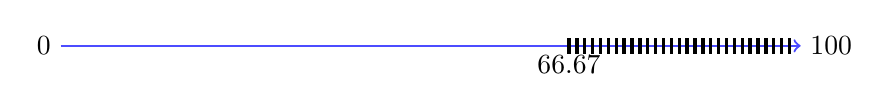
\begin{tikzpicture}
        \node (0) at (0, 0) {0};
        \node (100) at (10, 0) {100};
        \draw [->, thick, blue!70] (0) to (100);
        \node [below] (66) at (6.67, 0) {66.67};

        \foreach \x in {6.67,6.77,...,9.57}
        {
            \draw [very thick, black] (\x, -.1) to (\x, .1);
        }
    \end{tikzpicture}
\end{frame}


\begin{frame}
    \begin{center}
        \includegraphics[width=.8\textwidth]{./static/two_thirds_of_the_average_game/history_of_play/main.pdf}
    \end{center}
\end{frame}

\note{
    We see that over the two guesses the behaviour shifts.

    Note that with the first guesses: most people were above the winning guess.

    For the second guess: most people were below the winning guess.

    Will we eventually arrive at the equilibrium?
}

\begin{frame}
    \begin{center}
        \includegraphics[width=.8\textwidth]{./static/two_thirds_of_the_average_game/linear_regression_of_play/main.pdf}
    \end{center}
\end{frame}

\note{
    One approach would be to model the macro behaviour with that fitted line: if
    we assume that the $n+1$th guess is $.22$ of the $n$th guess we could
    imagine that this would eventually converge. We'd need more data here of
    course.

    This does not necessarily work, perhaps, as most players in the second guess
    were below the winning guess, a third guess would in fact be higher! So
    perhaps the linear regression would not longer be accurate.

    Let us base our analysis on biological evolution.
}

\section{Replicator dynamics}

\begin{frame}
    \begin{definition}{Replicator Dynamics Equation}
        \[\frac{dx_i}{dt}=x_i(f_i(x) - \phi)\text{ for all }i\]

        where: 

        \[\phi=\sum_{i=0}^Nx_if_i(x)\]
    \end{definition}
\end{frame}

\note{
    This differential equation ensures that individuals with a fitness above
    the average \(\phi\) have positive derivative and individuals with a fitness
    below the average \(\phi\) have negative derivate.

    For the case of the two thirds game we can solve the differential equations
    numerically efficiently.

}

\begin{frame}
    \[
        f_i(x) = \frac{1}{1 + \left(i - \frac{2}{3}\sum_{i=0}^{N}ix_i\right) ^ 2}
    \]
\end{frame}

\begin{frame}
    \begin{center}
        \Large
        Results
    \end{center}
\end{frame}


\frame{
    \begin{block}{}
        An evolutionary game theoretic model of rhino horn devaluation\footfullcite{glynatsi2018}
    \end{block}
    \centering
    \includegraphics[width=.6\textwidth]{./static/rhino.jpg}
}

\note{
    There are numerous examples of applications of evolutionary game theory. In
    this particular paper, my co-authors and I modelled the practice of
    devaluing a Rhino's horn (either by dying it or cutting it off) to dissuade
    poachers.

    The logic behind this idea is that there is a best response by poachers
    which is to not kill a Rhino for its horn. However, using evolutionary game
    theory lets us understand if this is actually likely to happen.
}

\end{document}
